
%% bare_conf.tex
%% V1.3
%% 2007/01/11
%% by Michael Shell
%% See:
%% http://www.michaelshell.org/
%% for current contact information.
%%
%% This is a skeleton file demonstrating the use of IEEEtran.cls
%% (requires IEEEtran.cls version 1.7 or later) with an IEEE conference paper.
%%
%% Support sites:
%% http://www.michaelshell.org/tex/ieeetran/
%% http://www.ctan.org/tex-archive/macros/latex/contrib/IEEEtran/
%% and
%% http://www.ieee.org/

\documentclass[conference]{IEEEtran}

\usepackage{graphicx}
\usepackage{float}
\usepackage{color}
\usepackage{listings}
\usepackage{ipa}

\begin{document}

% ---------------------- TITLE ---------------------- %

\title{Comparing Application Semantics with S$^2$E \\ {\large Determining whether busybox and coreutils are actually the same}}
% or \title{Symbolically Executing Real Applications \\ {\large Trying to make S$^2$E work with real software}}

\author{\IEEEauthorblockN{Mariana D'Angelo}
\IEEEauthorblockA{Department of Electrical and Computer Engineering\\
University of Toronto\\
Toronto, Canada\\
mariana.dangelo@utoronto.ca}
\and
\IEEEauthorblockN{Dhaval Miyani}
\IEEEauthorblockA{Department of Electrical and Computer Engineering\\
University of Toronto\\
Toronto, Canada\\
dhaval.miyani@utoronto.ca}}

\maketitle

% ---------------------- INTRODUCTION ---------------------- %

\section{Introduction}

While the key idea behind symbolic execution arose almost forty
years ago \cite{select}, it has only recently become practical due to
advances in constraint satisfiability \cite{satisfiability} and scalable approaches
with mixed symbolic and concrete execution \cite{systems-crash, dart}.
A 2011 study has shown that symbolic execution tools are beginning to
be used increasingly in industrial practice at corporations such as Microsoft,
NASA, IBM, and Fujitsu \cite{symb-ex-practice}. This proliferation shows the
importance of new symbolic execution tools and the impact they will have
on the industry as they improve.

S$^2$E is a symbolic execution platform that can operate directly on application
binaries for analyzing the properties and behaviour of software systems. It
analyzes programs in-vivo (the whole environment) within a real software stack
(user program, libraries, kernel, drivers, etc.) rather than using abstract models
of these layers. It is commonly used for performance profiling, reverse engineering
of proprietary software, and finding bugs in user-mode and kernel-mode
binaries \cite{s2e}. S$^2$E is a complex system due to the rich features it has
(particularly the fact that it runs inside of a VMM). This complexity, however, comes
with the price of being difficult to start using on existing software.

The goal of this experiment is to understand how a complex system such
as S$^2$E can be applied to existing software and document the process.
In particular, we are interested in seeing whether program inputs and code
need to be sanitized in some way to become amenable to dynamic analysis
via symbolic execution. Taking inspiration from KLEE \cite{klee}, we will be
comparing the semantics of two implementations of (supposedly) the exact
same suite of programs: the GNU Coreutils utility suite and the Busybox
embedded system suite.

Comparing the semantics of two implementations can have many real world
applications. In the field of computer security, for example, the ability to compare
the semantics of a software compiled from source with a pre-compiled binary
could reveal malicious or accidental backdoors. In particular, the fact that S$^2$E
runs in a VMM would allow for it to be used to test kernel level programs such as
file systems (or compare read and write operations different file systems).

We have encountered several challenges in using the S$^2$E platform; one
in particular forced us to change the initial goal of our experiment (evaluating
two consistency models from S$^2$E) due to the fact that not all of the six
consistency models described in \cite{s2e} are actually implemented in the
platform. Our biggest challenge with this project was trying to modify the programs
of interest in such a way that they could be directly comparable. The different
approaches we tried will be thoroughly discussed in the Experiments section of this
paper along with our own explanations about why they failed or succeeded and
what impact these choices had on the program analysis as a whole.

This paper is organized as follows: Section II presents some background regarding
symbolic execution, Section III discusses our approach to the experiments, Section IV 
describes in detail how we attempted to implement our approach, Section V discusses 
the results of our successful experiment with echo, Section VI presents the status 
of our implementation, Section VII concludes with some lessons learned, and finally in
Section VIII we discuss future work. 

% ---------------------- BACKGROUND ---------------------- %

\section{Background}

There is much work in symbolic execution for testing \cite{klee, RWset, vul-signature, system-crash, exe, bad-input, end-to-end, dyn-test, compositional-test, dart, sage, cute}. A typical approach for testing is fuzzing \cite{sage}, which involves generating random inputs for a program in an attempt to exercise all paths in a program (and hopefully hit any buggy code). This is known as concrete execution which involves running the program with deterministic values. Fuzz testing has several limitations, in particular coverage of paths in a program. For example, Listing \ref{code-fuzzing} shows a if statement which is only taken when x is 10. There are $2^{32}$ possible values which x could take when an input is randomly generated and as such the probability of actually taking this path is $2^{-32}$. This example demonstrates that the likelihood of some paths being taken when fuzzing is extremely low, which is the reason for the poor test coverage of concrete execution.

%  ------ CODE SYNTAX HIGHLIGHTING ------ %

\definecolor{mygreen}{rgb}{0,0.6,0}
\definecolor{myblue}{rgb}{0,0,0.6}
\definecolor{mymauve}{rgb}{0.58,0,0.82}
\definecolor{myred}{rgb}{0.6,0,0}
\definecolor{gray}{rgb}{0.5,0.5,0.5}
\definecolor{mygray}{gray}{0.25}

\lstdefinestyle{C}{
	language=C,
	xleftmargin=10pt,
	xrightmargin=0pt,
	basicstyle=\footnotesize\bfseries\ttfamily,
	showspaces=false,
	showtabs=false,
	breaklines=true,
	showstringspaces=false,
	breakatwhitespace=true,
	commentstyle=\color{mygreen},
	keywordstyle=\color{myblue},
	stringstyle=\color{myred},
	numbers=left,
	numbersep=5pt,
	numberstyle=\footnotesize\color{mygray},
	tabsize=4,
	frame=TB,
	framesep=5pt,
	escapeinside={\%*}{*}
}

\lstdefinestyle{Lua}{
	xleftmargin=10pt,
	xrightmargin=0pt,
	basicstyle=\footnotesize\bfseries\ttfamily,
	showspaces=false,
	showtabs=false,
	breaklines=true,
	showstringspaces=false,
	breakatwhitespace=true,
  	morecomment=[l]{--}, % single line comments
	morestring=[b]",% backslash escaped strings
	commentstyle=\color{mygreen},
	keywordstyle=\color{myblue},
	stringstyle=\color{myred},
	numbers=left,
	numbersep=5pt,
	numberstyle=\footnotesize\color{mygray},
	tabsize=4,
	frame=TB,
	framesep=5pt,
	escapeinside={\%*}{*}
}

\begin{lstlisting}[style=C, label=code-fuzzing, abovecaptionskip=2ex, captionpos=b, caption={Code example where fuzzing generally has poor coverage}]
if (x == 10) {
	// path 1
} else {
	// path 2
}
\end{lstlisting}

 Symbolic execution, on the other hand, runs the application with symbolic inputs \cite{klee} which are initially unconstrained by design. The program executes with these symbolic values and replaces concrete operations with ones that can manipulate symbolic values. The symbolic execution engine ``follows" both paths whenever it encounters a branch on a symbolic value and adds the path condition to a set of constraints known as the ``path constraint". When a bug is encountered in the code a test case (i.e., concrete inputs) can be generated from the path constraint. There are two main limitations of symbolic execution: (1) ``the path explosion problem" \cite{s2e}, which is due to the exponential growth of paths in a program caused by conditional branches, and (2) ``the environment problem" \cite{klee}, which is due to interactions with the surrounding environment (e.g, operating system, network, etc.).

 In order to deal with the environment problem, one can use a mixture of symbolic and concrete execution (also known as concolic execution \cite{cute}). Concolic execution gathers constraints using symbolic execution, but then generates concrete values using a constraint solver in order to address the environment problem. Once these concrete values are generated the program can interact with its environment in a normal fashion without the overheads and problems associated with symbolically executing the environment.

S$^2$E is a symbolic execution engine which can perform concrete execution, symbolic execution, and concolic execution depending on the consistency model chosen. There are six different consistency models in S$^2$E, described below. Figure \ref{s2e-cm} provides an overview of the models showing how they transition from highly strict to highly relaxed models with some details about what consistency requirements are relaxed for each model. A model is consistent if there exist a globally feasible path through the system for every path explored in the unit. A unit is the block one wishes to analyze and the environment is the rest of the system.

\begin{itemize}
\item \textit{Strictly Consistent Concrete Execution (SC-CE):}
No symbolic execution in unit or environment.
\item \textit{Strictly Consistent Unit-level Execution (SC-UE):}
Unit is symbolically executed while the
environment is executed concretely.
\item \textit{Strictly Consistent System-level Execution
(SC-SE):} Unit and environment are executed
symbolically - this is the only model that
executes the environment symbolically.
\item \textit{Local Consistency (LC):} Similar to SC-UE,
but it adheres to constraints that the
environment/unit API contracts impose on
return values.
\item \textit{Relaxed Consistency Overapproximate
Consistency (RC-OC):} Similar to LC, but it
ignores the constraints from the environment/unit API contracts.
\item \textit{Relaxed Consistency CFG Consistency (RC-CC):}
Similar to SC-UE, but like static analysis it can explore any
path in the unit's inter-procedural control flow graph (even
infeasible ones).
\end{itemize}

There are several differences between S$^2$E and other similar symbolic execution engines. For instance, KLEE uses file system models \cite{klee} to avoid symbolically executing the actual filesystem. S$^2$E does not take this approach as writing models is a labour intensive and error-prone process. Cute \cite{cute} executes the environment concretely (i.e., without modelling) with a consistency model similar to S$^2$E's SC-SE, but it is limited to code-based selection and one consistency model. S$^2$E does not use compositional symbolic execution \cite{compositional-test}, a performance optimization which saves results for parts of the program (e.g., a function) and reuses them when that part is called in a different context. With concolic execution everything runs concretely for full systems, however, when the execution crosses program boundaries it may result in lost paths \cite{s2e}. Due to this, KLEE and CUTE cannot track path conditions in the environment and hence are unable to re-execute calls to enable overconstrained but feasible paths (e.g., malloc does not execute deterministically). DART \cite{dart}, CUTE \cite{cute} and EXE \cite{exe} use mix-mode execution (concretely executing some parts and symbolically executing others) to increase efficiency, however, they do not use automatic symbolic-concrete bidirectional data conversion (i.e., automatic conversion between concrete and symbolic values at program boundaries such as the unit and the environment) unlike S$^2$E, which is key to S$^2$E's scalability and low programmer effort.

Static analysis is performed without executing the program in question and has known limitations such as a high false positive and negative rate (due to infeasible paths) \cite{sage} and a lack of runtime environment analysis (as only the application source code is parsed). To reduce the number of false positives tools such as Saturn \cite{saturn} and bddbddb \cite{bddbddb} use a path-sensitive analysis engine. Saturn aims to detect logic programming language bugs by summarizing functions. bddbddb finds buggy patterns in a database where programs are stored as relations. As can be inferred, these tools are language specific and require different implementations for different programming languages. Additionally, using these tools requires learning a new programming language. As a dynamic analysis framework, S$^2$E addresses the limitations of static analysis tools. For example, they directly operate on and analyze binaries whereas static analysis would require disassembly and decompilation. This could involve converting an x86 binary to the LLVM format and running it through an engine like KLEE. Disassembly and decompilation \cite{disassembly} are classically undecidable problems (e.g., disambiguating code from data) \cite{s2e}.

\begin{figure}[!t]
\centering
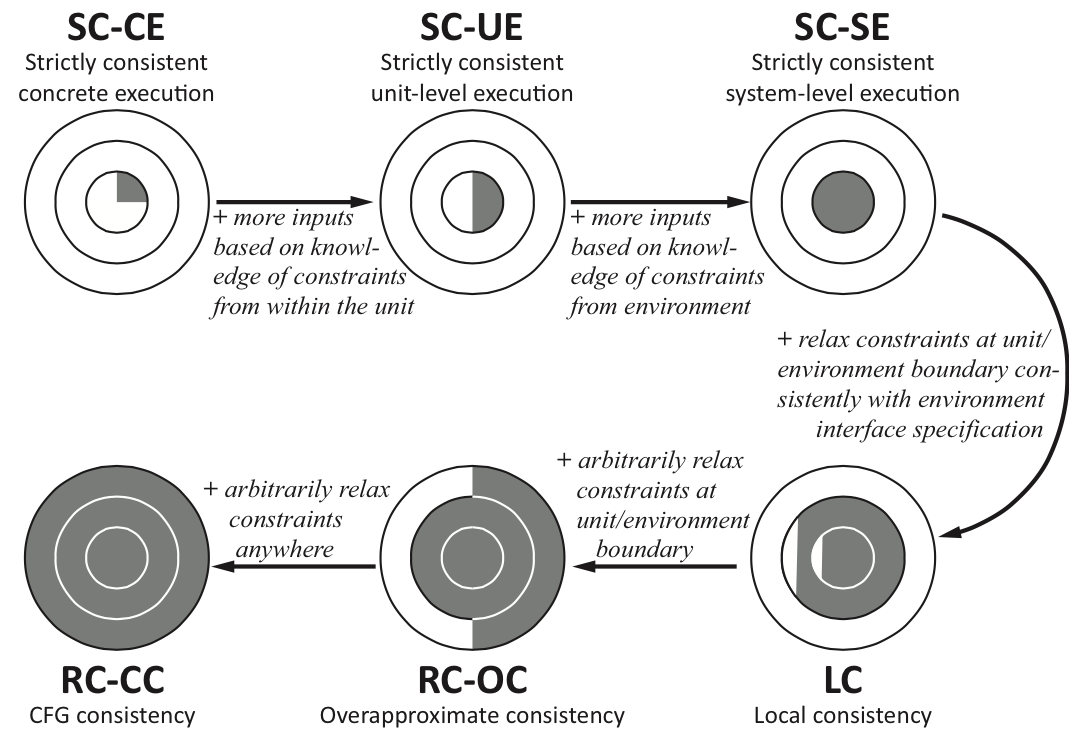
\includegraphics[width=3in]{s2e-consistency-models.png}
\caption{S$^2$E Consistency Models \cite{s2e}}
\label{s2e-cm}
\end{figure}

% ---------------------- APPROACH ---------------------- %

\section{Approach}

The high level approach we took to use S2E for equivalence testing was as follows:

\begin{enumerate}
  \item Run each program with symbolic input (using {\tt s2e\_make\_symbolic()} from a test application invoking the functions or directly on the binary with option {\tt --sym-args}).
  \item Compare the output of the Busybox and GNU Coreutils implementation of the same program using {\tt s2e\_assert}, which performs a regular assert but also does some cleaning up for S2E and generates sample input which violates the assertion.
  \item Using the sample input generated, manually analyze the two implementations (possibly using GNU Debugger) to identify semantic differences between the two implementations. 
\end{enumerate}

% ---------------------- IMPLEMENTATION ---------------------- %

\section{Implementation}

In this section we will describe all of the ways in which we tried to symbolically execute the two binaries (from GNU Coreutils and Busybox) to perform equivalence testing. 

\subsection{Running the binary directly}

Initially, we attempted to run the analysis directly on the binaries for the two implementations of echo - having built the two utility suites precisely as suggested by the developers. These results, however, were not easily comparable and did not provide information regarding the semantic differences between the two implementations. From this attempt, it was apparent that running S$^2$E directly on a binary is better suited for simply testing an application with all possible inputs and high coverage, rather than determining semantic equivalence. \\

Listing \ref{s2e-binary} shows the command used to execute the binary of GNU Coreutils' {\tt echo}. In order to symbolically execute the binary we must pre-load the {\tt init\_env} library (line 1) which intercepts the programs entry point invocation, parses the command line program arguments and configures symbolic execution before invoking {\tt echo}'s main method. We also have to specify some options for our symbolic execution (line 2); {\tt --select-process-code} enables forking the only in the code portion of the current binary, and {\tt --sym-args 0 2 4} generates 0-2 symbolic arguments of length 4 for {\tt echo}. Finally, we use {\tt s2ecmd kill} (line 3) to kill the execution path once {\tt echo} returns to prevent S$^2$E from running forever. \\

\begin{lstlisting}[style=C, label=s2e-binary, abovecaptionskip=2ex, captionpos=b, caption={Command for symbolically executing the GNU Coreutils {\tt echo} binary with S$^2$E}]
LD_PRELOAD=/path/to/guest/init_env/init_env.so \
 /bin/echo --select-process-code --sym-args 0 \
 2 4 ; /path/to/guest/s2ecmd/s2ecmd kill 0 \
  "echo done"
\end{lstlisting}

\subsection{Executing the binary from within a tester program}

After determining that we would need to invoke both of the implementations from within the same program to compare their semantics, we elected to use the direct approach shown in Listing \ref{s2e-popen}. Here we created a symbolic variable x (lines 1 and 2), created the command to invoke {\tt echo} using {\tt snprintf} (line 3), then enabled S$^2$E's forking (line 5) before using {\tt popen} to execute the command (line 7). We could not use {\tt execv} here because we would not have been able to read what {\tt echo} wrote to stdout since {\tt execv} forks a new process, whereas {\tt popen} creates a pipe between the program and the command, and returns a pointer to a stream that can be read from. Later in the code (line 10), we used {\tt fread} to retrieve that stream and read its contents into a buffer. Unfortunately, this technique did not work because S$^2$E was symbolically executing {\tt popen} and so the analysis took too much time, consumed too much memory, and did not yield useful results. \\

\begin{lstlisting}[style=C, label=s2e-popen, abovecaptionskip=2ex, captionpos=b, caption={Code to symbolically invoke the GNU Coreutils {\tt echo} binary from a tester program}]
FILE* pipe; char command[70]; char x[2];
s2e_make_symbolic(&x, sizeof(x), "x"); // make x symbolic
int len = snprintf(command, sizeof(command), "echo %s", x);
if (len <= sizeof(command)) {
    s2e_enable_forking();
    pipe = popen(command, "r");
    s2e_disable_forking();
}
...
char buf[100];
fread(buf, 1, 1024, pipe);
\end{lstlisting}

\subsection{Creating libraries for each implementation}

[DHAVAL] Tried to make the echo implementations into shared libraries so they could be called directly from our test program (shared library vs. static library stuff) - make sure you discuss why we needed a shared/static library in the first place

\subsection{Redirecting stdout to a buffer}

Once we had successfully managed to invoke the two implementations of {\tt echo} from our tester program we needed to retrieve the output of the programs in order to compare their semantics. As both implementations write output directly to the shell we elected to redirect {\tt stdout} using the commands in Listing \ref{s2e-redirect}. Although this worked for GNU Coreutils, the invocation of Busybox's implementation of {\tt echo} caused our buffer to be corrupted. Upon investigation, we discovered that although GNU Coreutils uses {\tt stdio}, Busybox avoids using it as the developers do not assume that {\tt stdout} is actually open (and failed writes fill up the input buffer which cannot always be flushed), so they use {\tt writev} to output the result. \\ 

\begin{lstlisting}[style=C, label=s2e-redirect, abovecaptionskip=2ex, captionpos=b, caption={Code snippet for redirecting stdout to a buffer}]
char buf[128];
freopen("coreutils.out", "w", stdout);
setbuf(stdout, buf);
\end{lstlisting}

At this point we decided to simply write the result to a file (omitting lines 1 and 3 of Listing \ref{s2e-redirect}), which solved our corruption issues. However, when we tried to symbolically execute the program we discovered that S$^2$E was only executing concretely! Upon further inspection it became apparent that S$^2$E concretized the value of the buffer because our symbolic program argument was only being read from and not written to. Encountering this roadblock, we elected to look into KLEE's methodology for their comparison of the two utility suites. We discovered that KLEE was symbolically modelling stdout (command line option {\tt -sym-stdout}). Since S$^2$E is built upon KLEE we tried to add this flag into the {\tt kleeArgs} portion of the configuration file used by S$^2$E, however this option did not exist, most likely due to the fact that S$^2$E is intended as an in vivo platform that uses a real software stack (i.e., it avoid modelling parts of the system).

\subsection{Modifying the implementations to not use stdout}
[DHAVAL] Final approach: modifying coreutils echo and busybox echo to return a string instead of printing to stdout [SUCCESS!]

% ---------------------- EXPERIMENTS ---------------------- %

\section{Experiments}

For our experiment to check the semantic equivalence of two implementations of {\tt echo} we used GNU Coreutils version 8.23 and Busybox 1.22.1 (the latest versions at the time of this writing). The configuration file used to run S$^2$E is provided in Listing \ref{s2e-config} for reference. The use of the {\tt ExecutionTracer} on line 13 and the {\tt TestCaseGenerator} on line 16 were necessary to output the constraints for each state and generate concrete values for failed asserts, respectively. \\

\begin{lstlisting}[style=Lua, label=s2e-config, abovecaptionskip=2ex, captionpos=b, caption={S$^2$E configuration file used for experiment}]
-- File: config.lua
s2e = {
  kleeArgs = {
    --Switch states only when the current one terminates
    "--use-dfs-search"
  }
}
plugins = {
  -- Enable S2E custom opcodes
  "BaseInstructions",

  -- Basic tracing required for test case generation
  "ExecutionTracer",

  -- Enable the test case generator plugin
  "TestCaseGenerator",
}

pluginsConfig = {}
\end{lstlisting}

Once we made changes to both implementations of {\tt echo} to return strings rather than output the result and created shared/static libraries to invoke these functions from our equivalence checking program, we were able to run both programs symbolically and compare their results using the code in Listing \ref{s2e-equ}. One lines 8-9 we allocate the input character arrays on the heap due to [DHAVAL]. We then create an input variable x, make it symbolic, and add it to the input character array before enabling forking in S$^2$E (line 17). On lines 18-19 we call the two implementations of {\tt echo} (GNU Coreutils = {\tt printecho}, Busybox = {\tt printbbecho}), on line 21 we assert that the two implementations produce the same result, and on line 23 we kill the state (this code is only reached if the assert was true). \\

\begin{lstlisting}[style=C, label=s2e-equ, abovecaptionskip=2ex, captionpos=b, caption={Program used to perform equivalence testing on GNU Coreutils and Busybox}]
#include <stdlib.h>
#include <stdio.h>
#include <string.h>
#include "s2e.h"

int main() {
	char** str = malloc(2*sizeof(char*));
	str[0] = malloc(2*sizeof(char));
	str[1] = malloc(2*sizeof(char));
	memset(str[0], 0, 2);
	memset(str[1], 0, 2);

	unsigned char x[2];
	s2e_make_symbolic(&x, 2, "x");
	memcpy(str[1], x, 2);

	s2e_enable_forking();
	char * out1 = printecho(2, str);
	char * out2 = printbbecho(2, str);

	s2e_assert(memcmp(out1, out2, 2)==0);
    
	s2e_kill_state(0, "Success");
	return 0;
}
\end{lstlisting}

Our analysis produced the results similar to those shown in listing \ref{s2e-equiv-result} which provides the constraints for that state (lines 2-7 for state 6) and also a sample test case that satisfies those constraints (lines 29-31 for state 6). Such output exists for states that fail there assertion (state 6) as well those that exit normally (state 7). There were five assertion failures in our output falling under two categories: those that ended with {\tt 0x00} (i.e., the {\tt NULL} character), and those that ended with extended ASCII values like {\corner} (expressed as a signed integer -0x65). \\

Using the sample input provided by S$^2$E we manually analyzed the two implementations of {\tt echo} to see why their were differences. We determined that although both implementations of {\tt echo} print a space between strings found in {\tt argv}, the conditions leading to printing a space are different. In GNU Coreutils' implementation, if there is at least one string to echo (check {\tt argv {$>$} 0}) a space is added after the current word. Conversely, in Busybox's implementation a space is only printed after a string if there is another string to print after the current one (check {\tt *++argv !=  NULL}). \\

We also had a personal experience of S$^2$E finding a bug due to an implementation error when changing the implementation of GNU Coreutils' {\tt echo} to return a string rather than output the result. Here we had accidentally changed the code which prints a newline after the echo is completed with code to print a space. Luckily, S$^2$E was able to bring this error to our attention and we fixed this before running our actual experiments. \\

\begin{lstlisting}[style=C, label=s2e-equiv-result, abovecaptionskip=2ex, captionpos=b, caption={Partial output of equivalence testing for GNU Coreutils and Busybox}]
131 [State 6] Forking state 6 at pc = 0x804923a into states:
    state 6 with condition (Eq (w32 0)
    (And w32 (Add w32 (w32 4294967227)
        (Concat w32 (w8 0)
            (Concat w24 (w8 0)
                (Concat w16 (w8 0) (Read w8 1
                    v0_x_0))))) (w32 255)))
    state 7 with condition (Not (Eq (w32 0)
    (And w32 (Add w32 (w32 4294967227)
        (Concat w32 (w8 0)
            (Concat w24 (w8 0)
                (Concat w16 (w8 0) (Read w8 1 
                    v0_x_0)))))(w32 255))))
...
131 [State 6] Switching from state 6 to state 7
132 [State 7] Killing state 7
132 [State 7] Terminating state 7 with message 'State was terminated by opcode
            message: "Success"
            status: 0'
TestCaseGenerator: processTestCase of state 7 at address 0x8048cb9

v0_x_0: 2d -30 0
132 [State 7] Switching from state 7 to state 6
...
132 [State 6] Killing state 6
132 [State 6] Terminating state 6 with message 'State was terminated by opcode
            message: "Assertion failed: memcmp(out1, out2, 2)==0"
            status: 0'
TestCaseGenerator: processTestCase of state 6 at address 0x8048cb9

v0_x_0: 2d -45 E
\end{lstlisting}

% ---------------------- STATUS ---------------------- %

\section{Status}

[DHAVAL] Current status of implementation.

\begin{itemize}
  \item After several failed attempts we decided to modify the utilities and got S2E working with both implementations of echo.
\end{itemize}

% ---------------------- CONCLUSION ---------------------- %

\section{Conclusion}

[DHAVAL] Did your results meet expectations?

\begin{itemize}
	\item Summarize intro (what did we do, why did we do it)
  \item Lessons learned: lack of documentation and an incomplete understanding of how S2E symbolically executes led to a lot of mistakes.
\end{itemize}

% ---------------------- FUTURE WORK ---------------------- %

\section{Future Work}

[DHAVAL]

\begin{itemize}
  \item Perform these tests on the rest of the utilities in busybox and gnu coreutils.
  \item Try testing other programs that don't use stdout and determine if they present any different challenges.
  \item Figure out how to change the VMM parameters for S2E (e.g., give it more memory). Discuss how even building from source had its problems as we could not transfer files from host to guest when we built S2E manually.
\end{itemize}

% ---------------------- BIBLIOGRAPHY ---------------------- %

\begin{thebibliography}{1}

\bibitem{s2e}
CHIPOUNOV, V., GEORGESCU, V., ZAMFIR, C., AND CANDEA, G
Selective symbolic execution. In Workshop on Hot Topics
in Dependable Systems, 2009.

\bibitem{symb-ex-practice}
CADAR, C., GODEFROID, P., KHURSHID, S., PASAREANU, C., SEN, K., TILLMANN, N., AND VISSER, W.
Symbolic execution for software testing in practice � preliminary assessment. In ICSE Impact�11, May 2011.

\bibitem{select}
BOYER, R. S., ELSPAS, B., AND LEVITT, K. N.
SELECT - a formal system for testing and debugging programs by symbolic execution.
SIGPLAN Not., 10:234�245, 1975.

\bibitem{satisfiability}
DE MOURA, L. AND BJ�RNER, N.
Satisfiability modulo theories: introduction and applications.
Commun. ACM, 54:69�77, Sept. 2011.

\bibitem{systems-crash}
CADAR, C. AND ENGLER, D.
Execution generated test cases: How to make systems code crash itself.
In SPIN�05, Aug 2005.

\bibitem{klee}
CADAR, C., DUNBAR, AND ENGLER, D.R.
KLEE: Unassisted and automatic generation of high-coverage tests
for complex systems programs. In Symp. on Operating Systems
Design and Implementation, 2008.

\bibitem{cute}
SEN, K., MARINOV, D., AND AGHA, G. CUTE: A concolic unit testing engine for C. In In 5th joint meeting of the European Software Engineering Conference and ACM Symposium on the Foundations of Software Engineering (ESEC/FSE 2005).

\bibitem{RWset}
BOONSTOPPEL, P., CADAR, C., AND ENGLER, D. RWset: At- tacking path explosion in constraint-based test generation. In Proceedings of Tools and Algorithms for the Construction and Analysis of Systems (TACAS 2008).

\bibitem{vul-signature}
BRUMLEY, D., NEWSOME, J., SONG, D., WANG, H., AND JHA, S. Towards automatic generation of vulnerability-based sig- natures. In Proceedings of the 2006 IEEE Symposium on Security and Privacy (IEEE S\&P 2006).

\bibitem{system-crash}
CADAR, C., AND ENGLER, D. Execution generated test cases: How to make systems code crash itself. In Proceedings of the 12th International SPIN Workshop on Model Checking of Soft- ware (SPIN 2005).

\bibitem{exe}
CADAR, C., GANESH, V., PAWLOWSKI, P., DILL, D., AND ENGLER, D. EXE: Automatically generating inputs of death. In Proceedings of the 13th ACM Conference on Computer and Communications Security (CCS 2006).

\bibitem{bad-input}
COSTA, M., CASTRO, M., ZHOU, L., ZHANG, L., AND PEINADO, M. Bouncer: Securing software by blocking bad input. In Proceedings of the 21th ACM Symposium on Operating Systems Principles (SOSP 2007).

\bibitem{end-to-end}
COSTA, M., CROWCROFT, J., CASTRO, M., ROWSTRON, A., ZHOU, L., ZHANG, L., AND BARHAM, P. Vigilante: end-to-end containment of Internet worms. In Proceedings of the 20th ACM Symposium on Operating Systems Principles (SOSP 2005).

\bibitem{dyn-test}
EMMI, M., MAJUMDAR, R., AND SEN, K. Dynamic test input generation for database applications. In International Symposium on Software Testing and Analysis (ISSTA 2007).

\bibitem{compositional-test}
GODEFROID, P. Compositional dynamic test generation. In Proceedings of the 34th Symposium on Principles of Programming Languages (POPL 2007).

\bibitem{dart}
GODEFROID, P., KLARLUND, N., AND SEN, K. DART: Directed automated random testing. In Proceedings of the Conference on Programming Language Design and Implementation (PLDI 2005).

\bibitem{sage}
GODEFROID, P., LEVIN, M. Y., AND MOLNAR, D. Automated whitebox fuzz testing. In Proceedings of Network and Distributed Systems Security (NDSS 2008).

\bibitem{disassembly}
SCHWARZ, B., DEBRAY, S., AND ANDREWS, G. Disassembly of executable code revisited. In Working Conf. on Reverse Engineering, 2002.

\bibitem{saturn}
DIILLIG, I., DILLIG, T., AND ALKEN, A. Sound, complete and scalable path- sensitive analysis. In Conf. on Programming Language Design and Implementation, 2008.

\bibitem{bddbddb}
LAM, M. S., WHALEY, J., LIVSHITS, V. B., MARTIN, M. C., AVOTS, D., CARBIN, M., AND UNKEL, C. Context-sensitive program analysis as
database queries. In Symp. on Principles of Database Systems, 2005.

\end{thebibliography}

% that's all folks
\end{document}
